\documentclass[times, 12pt, utf8]{book}
\usepackage[a4paper, top=2.5cm, bottom=2.5cm, left=2.5cm, right=2.5cm]{geometry}

\usepackage[utf8]{inputenc}
\usepackage[croatian]{babel}
\usepackage{amsmath}
\usepackage{array}
\usepackage{graphicx}
\usepackage{hyperref}
\usepackage{listings}

\pagestyle{plain}

% razmak izmedju odlomaka
\parskip 7.2pt

\renewcommand*\lstlistingname{Ispis}
\lstset{
language=C,
frame=single,
keywordstyle=\ttfamily,
breaklines=true,
basicstyle=\ttfamily,
numbers=left,
numberstyle=\tiny,
stepnumber=1,
numbersep=5pt,
tabsize=2,
captionpos=b,
breaklines=true,
breakatwhitespace=false,
showspaces=false,
showtabs=false,
showlines=true, % inace brise prazne retke s kraja
columns=flexible,
aboveskip=15pt,
}

\hypersetup{
colorlinks=true,
linkcolor=blue,
} 


% kod koji brise "Poglavlje" ispred naslova svakog poglavlja
\makeatletter
\renewcommand{\@makechapterhead}[1]{%
\vspace*{50 pt}%
{\setlength{\parindent}{0pt} \raggedright \normalfont
\bfseries\Huge
\ifnum \value{secnumdepth}>1 
   \if@mainmatter\thechapter.\ \fi%
\fi
#1\par\nobreak\vspace{40 pt}}}
\makeatother

\title{
\vfill
Upute za izradu laboratorijskih vježbi iz predmeta\\
\emph{Prevođenje programskih jezika}\\
\vspace{70pt}
}

\author{
\emph{Autori:}\\
Ivan Budiselić, Ivan Žužak
}
\date{
\vspace{30pt} 
\emph{Datum posljednje izmjene:}\\
\today
\vfill
Fakultet elektrotehnike i računarstva\\
Zavod za elektroniku, mikroelektroniku, inteligentne i računalne sustave
}



\begin{document}
\maketitle

% kod koji mice prazne stranice prije pocetka chaptera ako chapter ne pocinje na parnoj stranici
\let\cleardoublepage\clearpage

% ovo je nuzno da se izbjegne ruzno obojani ToC
\begingroup
\hypersetup{linkcolor=black}
\tableofcontents
\endgroup

\chapter{Uvod}
Ovaj dokument namijenjen je studentima predmeta \emph{Prevođenje programskih jezika} na Fakultetu elektrotehnike i računarstva.
U dokumentu je opisan zadatak laboratorijskih vježbi predmeta te organizacija, provedba i ocjenjivanje.

\section{Cilj laboratorijskih vježbi}
Studenti tijekom vježbi izrađuju vlastiti jezični procesor (preciznije, kompilator) s ciljem boljeg razumijevanja kako jezični procesor radi.
Kao rezultat laboratorijskih vježbi studenti predaju pojedine dijelove jezičnog procesora, a konačno i cijeli jezični procesor.

Kako bi se projekt izrade jezičnog procesora najviše moguće naslonio na prethodno znanje stečeno u dosadašnjem tijeku studija, jezični procesor koji će se izrađivati na laboratorijskim vježbama treba prevoditi zadani podskup jezika \emph{C} u mnemonički jezik procesora FRISC.
Prevedeni programi moći će se izvoditi na simulatoru koji će biti dostupan na stranicama predmeta prije početka rada na generiranju FRISC koda.

Jezični procesor neće imati grafičko korisničko sučelje, nego će s korisnikom komunicirati putem standardnog ulaza i izlaza kao što je i uobičajeno.

\section{Grupe za laboratorijske vježbe}
Studenti laboratorijske vježbe rade u grupama.
Svaki student u grupi praktično izrađuje neke dijelove jezičnog procesora prema dogovoru unutar grupe, ali mora biti upoznat sa svim dijelovima jezičnog procesora.
Grupu vodi jedan od studenata, a rad voditelja nadziru asistenti.
Voditelj grupe u pravilu se bira na temelju rezultata iz predmeta \emph{Uvod u teoriju računarstva} prethodne akademske godine.

\section{Odabir jezika izgradnje jezičnog procesora}
Svaka grupa za jezik izgradnje jezičnog procesora, tj.~programski jezik u kojem će jezični procesor grupe biti ostvaren, bira između jezika \emph{C}, \emph{C++}, \emph{Java}, \emph{C\#} i \emph{Python} (2.x ili 3.x).
\emph{C\#} rješenja prevodit će se kompilatorom iz \href{http://www.mono-project.com/What_is_Mono}{Mono platforme} i izvodit će se na Mono platformi\footnote{Neće biti moguće predati \emph{Visual Studio} projekt, nego će se organizacija rješenja morati prilagoditi u skladu s uputama koje su dane za svaku pojedinu vježbu.}.
Ako niste sigurni koji programski jezik odabrati, vjerojatno je najsigurniji izbor \emph{Java}.

Pretpostavka je da iz položenih predmeta na nižim godinama studija svi studenti koji pristupaju laboratorijskim vježbama znaju \emph{C}.
Ipak, \emph{C} u praksi predmeta nije čest odabir za jezik izgradnje.
Prvenstveni razlog za to je što je čak i jednostavan jezični procesor relativno složen program koji nužno koristi strukture podataka koje dinamički rastu.
To pak zahtijeva intenzivno korištenje dinamičke alokacije memorije i pokazivača što može izazvati dosta poteškoća.
Ako vam se čini da bi najbolji izbor za vašu grupu bio \emph{C}, razmislite o korištenju jezika \emph{C++}.
\emph{C++} podržava više programskih paradigmi te se kao takav može koristiti i u proceduralnom stilu kao \emph{C}, bez primjene objektno orijentirane paradigme.
Međutim, \emph{C++} u standardnoj biblioteci sadrži većinu struktura podataka koje će vam trebati u izgradnji jezičnog procesora te omogućiti u velikoj mjeri ili potpuno izbjegavanje dinamičke alokacije memorije i rada s pokazivačima.

\section{Provedba laboratorijskih vježbi}
Provedba laboratorijskih vježbi organizirana je u četiri laboratorijske cjeline te završnu predaju ostvarenog jezičnog procesora.
U svakoj laboratorijskoj cjelini grupa izrađuje zadani dio jezičnog procesora te ostvareno predaje na računalno ocjenjivanje ili na predajli laboratorijske vježbe objašnjava izgradnju i prikazuje rad ostvarenog dijela, ovisno o cjelini.
Zadaci za pojedine laboratorijske cjeline detaljno su opisani u kasnijim poglavljima, a dijele se na:

\begin{description}
\itemsep 1pt
\item[I laboratorijska cjelina:] izgradnja leksičkog analizatora
\item[II laboratorijska cjelina:] izgradnja sintaksnog analizatora
\item[III laboratorijska cjelina:] izgradnja semantičkog analizatora
\item[IV laboratorijska cjelina:] izgradnja generatora ciljnog programa
\end{description}

Završna predaja ostvarenog jezičnog procesora uključuje predaju izvornog koda i izvodive verzije ostvarenog jezičnog procesora.

Studenti tijekom izgradnje jezičnog procesora mogu konzultirati asistente koji vode laboratorijske vježbe, e-mailom ili na konzultacijama.

\section{Kako pripremiti rješenje laboratorijskih vježbi za računalno ocjenjivanje}
Za potrebe računalnog ocjenjivanja, vaše rješenje će s ispitnim sustavom komunicirati putem \emph{standardnog ulaza} (\emph{stdin}) i \emph{standardnog izlaza} (\emph{stdout}).
Ispitni sustav će pri pokretanju programa na standardni ulaz preusmjeriti odgovarajuću ulaznu datoteku i standardni izlaz preusmjeriti u datoteku koja će se onda uspoređivati s očekivanim izlazom.
Iz tog razloga od presudne je važnosti da se vaš program strogo drži formata ispisa zadanog za pojedinu vježbu i da na standardni izlaz ne ispisuje ništa osim onog što se traži.
Za sav ostali ispis (npr.~ispis grešaka korisniku ili ispis za praćenje rada programa) koristite standardni izlaz za greške (\emph{stderr}).

Zadnji znak u svakoj ulaznoj datoteci bit će znak novog retka i zadnji znak svakog ispisa treba biti znak novog retka.
Drugim riječima, kada ispisujete očekivani izlaz, nakon sadržaja svakog retka treba staviti znak novog retka.
Na primjer, pretpostavimo da program tijekom rada u niz (engl. \emph{array}) upiše \texttt{n} cijelih brojeva tipa \texttt{int}, koje treba ispisati jednog po retku.
Tada bi u jeziku \emph{C} algoritam za ispis izgledao kao u isječku \ref{lst:ispis_algoritam}.

\begin{lstlisting}[caption={Primjer algoritma za ispis.},label=lst:ispis_algoritam]
for (i=0; i<n; i++) {
    printf("%d\n", A[i]);
}
\end{lstlisting}

Smisao ovog primjera i prethodnog odlomka je da uočite da i nakon zadnjeg broja dolazi znak novog retka.

Ulazne datoteke će uvijek biti zadane u točno onakvom formatu kao što je opisano u ovom dokumentu, tj.~nije potrebno provjeravati je li ulaz ispravno formatiran i ispisivati greške u suprotnom.

Nadalje, \textbf{testirajte svoja rješenja} prije predaje.
To što program radi za primjere koje ćete naći u ovoj uputi ne mora značiti da je program točan.
Iako se ova tvrdnja čini očita, čest je slučaj da studenti predaju rješenja koja uopće nisu testirana i sadrže elementarne greške koje su se lako mogle ukloniti već i uz malo testiranja nad vlastitim primjerima.


\chapter{Prva laboratorijska vježba}\label{chap:I}
Tema prve laboratorijske vježbe je leksička analiza.
Grupe izrađuju generator leksičkog analizatora sličan programu Lex.
U nastavku je opisano kako generator leksičkog analizatora i generirani leksički analizator trebaju raditi i dani su savjeti za implementaciju.
Ova uputa pretpostavlja da je čitatelj upoznat sa ispredavanim gradivom o leksičkoj analizi.
S obzirom na opsežnost uputa, preporuča se jednom ih pročitati od početka do kraja, a nakon toga se upute mogu koristiti kao referenca prilikom implementacije.

Ukupni rezultat laboratorijskih vježbi bit će jezični procesor koji prevodi podskup jezika \emph{C} u mnemonički jezik procesora FRISC.
U prvoj laboratorijskoj vježbi izrađuje se relativno općeniti generator leksičkog analizatora koji će se onda iskoristiti i za generiranje leksičkog analizatora za zadani podskup jezika \emph{C}.
Nakon završetka sve četiri laboratorijske vježbe, grupe će generirani leksički analizator povezati s ostalim dijelovima u cjeloviti jezični procesor.

Na prvoj laboratorijskoj vježbi izrađuje se \emph{generator} leksičkog analizatora umjesto specijaliziranog leksičkog analizatora za podskup jezika \emph{C}.
Za leksički složene jezike, a tu se prvenstveno misli na dozvoljeni slobodan način zapisa ulaznog programa, izgradnja specijaliziranog leksičkog analizatora nije bitno lakša od izgradnje donekle općenitog generatora leksičkog analizatora.
S druge strane, izgradnja generatora daje bolji uvid u način rada leksičke analize bilo kojeg programskog jezika.
Također, izgradnja generatora omogućuje bolje razumijevanje i uspješnije korištenje postojećih profesionalnih generatora leksičkih analizatora.

\section{Generator leksičkog analizatora}

\begin{figure}[htb!]
\centering
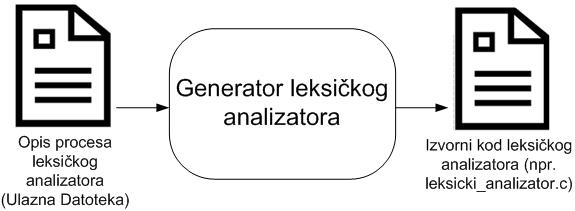
\includegraphics[width=0.7\textwidth]{slike/generator-leksickog-analizatora.jpg}
\caption{Način rada generatora leksičkog analizatora.}
\label{fig:generator-leksickog-analizatora}
\end{figure}

Način rada generatora leksičkog analizatora prikazan je slikom \ref{fig:generator-leksickog-analizatora}.
Generator leksičkog analizatora na standardnom ulazu dobiva opis procesa leksičkog analizatora.
Opis procesa leksičkog analizatora zadan je tekstualnom datotekom (dalje Ulazna Datoteka)\footnote{U skladu s napomenama u uvodu, ostvareni generator leksičkog analizatora treba čitati opis procesa leksičkog analizatora sa standardnog ulaza, a Ulazna Datoteka se onda preusmjerava na standardni ulaz prilikom pokretanja generatora.}.
Izlaz iz generatora leksičkog analizatora treba biti izvorni kod leksičkog analizatora napisan u jeziku izgradnje.
Ulazna Datoteka bit će zadana u sljedećem formatu:
\begin{description}
\itemsep 1pt
\item \emph{regularne definicije}
\item \%X \emph{stanja leksičkog analizatora}
\item \%L \emph{imena leksičkih jedinki}
\item \emph{pravila leksičkog analizatora}
\end{description}
U nastavku je objašnjeno kako pojedini dio datoteke izgleda.

\subsection{Regularne definicije}
Regularne definicije čine nadgradnju nad regularnim izrazima sa ciljem jednostavnijeg i preglednijeg opisa nekog regularnog jezika.
Regularne definicije opisane su u udžbeniku predmeta “Uvod u teoriju računarstva” \cite[poglavlje 2.3.2]{utr}.
U nastavku su opisani regularni izrazi i oblik regularnih definicija koje će se koristiti u Ulaznoj Datoteci.

\subsubsection*{Oblik regularnih izraza}
Kako bi se pojednostavio postupak pretvorbe regularnih izraza koji se koriste za definiciju leksičkih jedinki u konačni automat, svi regularni izrazi u Ulaznoj Datoteci koristit će isključivo:
\begin{itemize}
\itemsep 1pt
\item izbor podizraza koristeći operator \verb=|=
\item nadovezivanje (slijedno napisani znakovi ili grupe znakova, bez posebnog operatora)
\item Kleenove operator ponavljanja \verb=*= (ponavljanje nula ili više puta)
\item grupiranje koristeći oble zagrade \verb=(= i \verb=)=
\end{itemize}

Kao što je uobičajeno, prednost operatora ponavljanja \verb=*= veća je od prednosti nadovezivanja, a prednost nadovezivanja veća je od prednosti operatora izbora \verb=|=.
Odgovarajuća interpretacija regularnog izraza koja nije u skladu s ovim prednostima, može se postići grupiranjem koristeći zagrade.

Dodatno, zbog jednostavnosti, za prazan niz \(\varepsilon\) će se koristiti znak \verb=$= (dolar).
Zbog toga nigdje u regularnom izrazu neće biti praznih podizraza (npr. \verb=a||b= će biti zapisano kao \verb=a|$|b=).
U izrazima se neće pojaviti uzastopni operatori ponavljanja (na primjer \verb=a**=).

\subsubsection*{Regularne definicije u Ulaznoj Datoteci}
U Ulaznoj Datoteci bit će jedna regularna definicija po retku, sljedećeg oblika:\\
\verb|{|\emph{imeRegularneDefinicije}\verb|}|\textvisiblespace\emph{regularniIzraz}

Pritom, \emph{imeRegularneDefinicije} može sadržavati mala i velika slova engleske abecede, a \emph{regularniIzraz} je regularni izraz oblika u skladu s prije opisanim pravilima pri čemu osim pojedinačnih znakova smije sadržavati i proizvoljan broj referenci na prethodno definirane regularne definicije (vidi primjer ispod).
Početni znak \verb|{| će se nalaziti u prvom stupcu određenog retka, a između znaka \verb|}| i početka regularnog izraza nalazit će se točno jedan razmak.
U području regularnih definicija u Ulaznoj Datoteci neće se nalaziti niti jedan prazan redak.

Na primjer, dio regularnih definicija u Ulaznoj Datoteci može izgledati ovako:

\begin{lstlisting}[caption={Primjer regularnih definicija u Ulaznoj Datoteci.},label=lst:regdef]
{oktalnaZnamenka} 0|1|2|3|4|5|6|7
{dekadskaZnamenka} {oktalnaZnamenka}|8|9
{hexZnamenka} a|b|c|d|e|f|{dekadskaZnamenka}|A|B|C|D|E|F
\end{lstlisting}

Kao što se vidi u zadnjem retku primjera u ispisu \ref{lst:regdef}, referenca na prethodno definiranu regularnu definiciju može se nalaziti bilo gdje u regularnom izrazu.

\subsection{Stanja leksičkog analizatora}
Za pojedine klase leksičkih jedinki nužno je promatrati lijevi kontekst, tj. dio ulaznog niza koji je pročitan prije podniza koji čini leksičku jedinku.
Jedan od načina praćenja lijevog konteksta koji se često koristi u leksičkim analizatorima su stanja leksičkog analizatora.

Za potrebe generatora leksičkog analizatora koji se gradi u sklopu prve laboratorijske vježbe, u Ulaznoj Datoteci će nakon zadnje regularne definicije biti redak u kojem su definirana stanja koja će koristiti leksički analizator.
Redak će započeti znakovima \verb=%X= i točno jednim razmakom, nakon kojeg slijedi niz jedne ili više oznaka stanja odvojenih točno jednim razmakom (vidi primjer ispod).
Oznake stanja će se sastojati od malih i velikih slova engleske abecede i započinjat će nizom \verb=S_= (to će ujedno biti jedino mjesto u imenu stanja na kojem će biti znak \verb=_= (engl. \emph{underscore})).
Prvo stanje navedeno nakon \verb=%X= je početno stanje leksičkog analizatora.
Na primjer, definicija stanja leksičkog analizatora može izgledati kao u ispisu \ref{lst:stanja}.

\begin{lstlisting}[caption={Primjer imena stanja u Ulaznoj Datoteci.},label=lst:stanja]
%X S_pocetno S_komentar S_unarniMinus
\end{lstlisting}

\subsection{Imena leksičkih jedinki}
Odmah u sljedećem retku nakon definicije stanja leksičkog analizatora, u Ulaznoj Datoteci nalazit će se redak koji definira imena leksičkih jedinki koje generirani leksički analizator treba koristiti.
Redak će započeti znakovima \verb=%L= i točno jednim razmakom, nakon kojeg slijedi niz jednog ili više imena leksičkih jedinki odvojenih točno jednim razmakom (vidi primjer ispod).
Imena leksičkih jedinki će se sastojati od malih i velikih slova engleske abecede i znakova \verb=_= (engl. \emph{underscore}).
Na primjer, definicija imena leksičkih jedinki može izgledati kao u ispisu \ref{lst:imena_jedinki}.

\begin{lstlisting}[caption={Primjer imena stanja u Ulaznoj Datoteci.},label=lst:imena_jedinki]
%L IDENTIFIKATOR brojcanaKonstanta znakovnaKonstanta OP_PLUS
\end{lstlisting}

\subsection{Pravila leksičkog analizatora}
Pravila leksičkog analizatora definiraju sve leksičke jedinke ulaznog jezika i definiraju na koji način će generirani leksički analizator pohraniti sve potrebne podatke vezane uz leksičku jedinku.
U Ulaznoj Datoteci će pravila leksičkog analizatora biti navedena nakon retka koji definira imena leksičkih jedinki u sljedećem obliku:\\
\verb=<=\emph{imeStanja}\verb=>=\emph{regularniIzraz}\\
\verb|{|\\
\emph{argumentiAkcije}\\
\verb|}|

U datoteci će biti proizvoljan broj pravila, jedno iza drugog bez praznih redaka između pravila.
\emph{imeStanja} odgovarat će nekom od stanja definiranih ranije i bit će okruženo znakovima \verb|<| i \verb|>|.
\emph{regularniIzraz} slijedit će neposredno nakon znaka \verb|>| (bez razmaka) i bit će u prethodno opisanom formatu.
U regularnom izrazu mogu se pojaviti imena definirana u regularnim definicijama okružena znakovima \verb|{| i \verb|}| (vidi primjer ispod).

\emph{Napomena: Sva pravila} leksičkog analizatora imat će zadano stanje na početku pravila.
Određeno pravilo je aktivno ako i samo ako se leksički analizator nalazi u odgovarajućem stanju (vidi savjete za implementaciju ispod).
Prvenstveni razlog za ovakvu definiciju pravila je uniformnost što omogućuje jednostavniju implementaciju.

U sljedećem retku definicije pravila nalazit će se znak \verb|{| koji započinje dio za definiciju argumenata akcije.
Svi retci argumenata akcije počet će u prvom stupcu i niti jedan neće započinjati znakom \verb|}|.
Završetak dijela argumenata akcije bit će jednoznačno određen retkom koji sadrži samo znak \verb|}|.
Argumenti akcije određuju što generirani leksički analizator treba učiniti kada prepozna odgovarajuću leksičku jedinku.
Svaka akcija imat će jedan do četiri argumenata, svaki u svom retku.
U prvom retku argumenata akcije uvijek će se nalaziti ime pripadne leksičke jedinke (jedno od imena definiranih ranije u Ulaznoj Datoteci) ili znak \(-\) (minus).
U slučaju da je u akciji navedeno ime leksičke jedinke, generirani leksički analizator treba zadanu leksičku jedinku dodati u odgovarajuće tablice i u tablice upisati početne vrijednosti za tu leksičku jedinku (ovo je detaljnije objašnjeno u odjeljku \ref{sec:leksicki_analizator} ove upute).
S druge strane, znak minus označava da pročitani dio ulaznog niza treba odbaciti i da ne predstavlja leksičku jedinku.
Odbacivanje će se koristiti za izbacivanje komentara, bjelina i slično.
Pojedine akcije imat će jedan do tri posebna argumenta koji redom omogućuju brojanje redaka, upravljanje stanjem leksičkog analizatora i razrješavanje nejednoznačnosti.

Prvi posebni argument je \verb|NOVI_REDAK| što označava leksičkom analizatoru da je u izvornoj datoteci programa koji se prevodi došlo do promjene retka.
Retci se broje kako bi jezični procesor mogao ispisivati korisne podatke o mjestu pogreške, i tijekom leksičke analize i tijekom ostalih faza rada.
Povećani broj retka odnosi se tek na sljedeću leksičku jedinku, tj.~ako akcija prepoznaje neku leksičku jedinku (u prvom retku argumenata akcije nalazi se neko ime leksičke jedinke, a ne znak \(-\)) i ima argument \verb|NOVI_REDAK|, za broj retka te leksičke jedinke zapisuje se stari broj retka, prije uvećanja.

Drugi posebni argument je \verb|UDJI_U_STANJE| \emph{imeStanja} kojim leksički analizator prelazi iz trenutnog stanja u stanje \emph{imeStanja}.
Niz znakova \emph{imeStanja} bit će odvojen od niza \verb|UDJI_U_STANJE| točno jednim razmakom.
Treći posebni argument je \verb|VRATI_SE| \emph{naZnak} koji određuje da se od pročitanih znakova u leksičku jedinku treba grupirati prvih \emph{naZnak} znakova, a ostali znakovi vraćaju se u ulazni niz, kao da nisu ni pročitani (vidi primjer).
Ova naredba je ekvivalentna naredbi \verb|yyless(naZnak)| u Lexu.
\emph{naZnak} će biti cijeli broj bez vodećih nula i bit će odvojen od niza \verb|VRATI_SE| točno jednim razmakom.
Svi posebni argumenti prikazani su u primjeru, uz dodatne komentare u savjetima za implementaciju.

\subsection{Specijalni znakovi}\label{sec:specijalni_znakovi}
Pojedini znakovi se u opisu regularnih definicija i regularnih izraza u pravilima leksičkog analizatora koriste kao posebne oznake.
Kako bi generirani leksički analizator mogao te iste znakove prepoznati u izvornom kodu programa koji se prevodi, nužno je uvesti sustav prefiksiranja (engl. \emph{escaping}).
Kao što je uobičajeno, specijalni znakovi prefiksiraju se znakom \verb|\| (engl. \emph{backslash}) da bi dobili svoje izvorno značenje.
Dodatno, kako bi se u regularnom izrazu mogao prepoznati i sam znak \verb|\|, on se također mora prefiksirati dodatnim znakom \verb|\| (vidi primjer ispod).
Specijalni znakovi koji se koriste u generatoru leksičkog analizatora su:\\
\verb=( ) { } | * $ \=

Osim ovih znakova, generator leksičkog analizatora mora u Ulaznoj Datoteci prepoznati i niz znakova \verb|\n| kao znak za novi redak i niz znakova \verb|\t| kao znak tab.
Dodatno, razmak ćemo označavati nizom \verb|\_| (\emph{backslash underscore}) kako bi Ulazna Datoteka bila čitljivija i kako nebi bilo problema s uređivačima teksta koji brišu razmake na krajevima redaka.

\subsection{Primjer}\label{sec:generator_primjer}
U primjeru je prikazana Ulazna Datoteka jednostavanog jezika za računanje matematičkih izraza.
Jezik podržava samo binarno oduzimanje i unarni minus pa ćemo ga zvati \emph{minusLang}.
Unarni minus može se pojaviti više puta uzastopce.
Podržani su samo cijeli brojevi u dekadskom, oktalnom ili heksadekadskom zapisu.
Grupiranje se ostvaruje korištenjem oblih zagrada.
Dozvoljen je slobodan način zapisa matematičkog izraza kroz više redaka i s proizvoljnim brojem praznina.
Također su dozvoljeni i komentari koji prolaze kroz proizvoljan broj redaka, a ograđeni su nizovima \verb=#|= i \verb=|#=.
Zbog jednostavnosti Ulazne Datoteke, u jeziku nije dozvoljeno da se komentar pojavi ispred unarnog minusa.

Primjer programa pisanog u zadanom jeziku prikazan je u ispisu \ref{lst:minusLang_primjer}.
Ulazna Datoteka za leksičku analizu ovog jezika mogla bi izgledati \href{https://github.com/fer-ppj/ppj-labosi/raw/master/res/lab1/minusLang.lan}{ovako}.

\begin{lstlisting}[caption={Primjer programa pisanog u jeziku \emph{minusLang}.},label=lst:minusLang_primjer]
#| ovo je primjer |#
3 -  -0x12 - ( #| ovdje ce doci grupirane
		operacije |#
3- -
--076) #| 3 - ---076 = 3 - -076 = 3 + 076 |#

\end{lstlisting}

U području regularnih definicija, definirana je jedinstvena definicija broja koja prihvaća zapis broja u sve tri baze (oktalne brojeve ne trebamo posebno definirati jer izgledaju kao dekadski s vodećom nulom).
To znači da leksička analiza neće razlikovati brojevne baze, odnosno neće provjeravati sadrži li oktalni broj znamenke \verb|8| ili \verb|9|, nego će te provjere odraditi neka kasnija faza rada jezičnog procesora, tipično semantička analiza\footnote{O ovom i sličnim pitanjima bit će govora na predavanjima predmeta tijekom semestra.}.

Na početku regularnog izraza definicije \verb|{sviZnakovi}| nalaze se svi specijalni znakovi, prefiksirani znakom \verb|\|, kao što je ranije opisano.
Izbacivanje komentara odrađuje se s četiri pravila prikazana u ispisu \ref{lst:minusLang_komentari}.

\begin{lstlisting}[caption={Pravila za izbacivanje komentara iz ulaznog programa.},label=lst:minusLang_komentari]
<S_pocetno>#\|
{
-
UDJI_U_STANJE S_komentar
}
<S_komentar>\|#
{
-
UDJI_U_STANJE S_pocetno
}
<S_komentar>\n
{
-
NOVI_REDAK
}
<S_komentar>{sviZnakovi}
{
-
}
\end{lstlisting}

Prva akcija prepoznaje početni niz znakova koji označava komentar.
Za prepoznavanje specijalnog znaka \verb=|= koristi se prefiks \verb|\|.
Slično, drugo pravilo pronalazi kraj komentara i vraća leksički analizator u početno stanje.
S obzirom na to da se komentari mogu provlačiti kroz proizvoljan broj redaka, nužno je i unutar stanja za prepoznavanje komentara nastaviti brojati retke.
Brojanje redaka ostvaruje trećim pravilom.
Konačno, u komentaru se može pojaviti mnogo znakova koji inače nisu dozvoljeni van komentara.
Važno je primijetiti da četvrto pravilo prepoznaje jedan po jedan znak unutar komentara koristeći regularnu definiciju \verb|{sviZnakovi}|.
Na taj način će biti moguće prepoznati niz znakova koji predstavlja kraj komentara (prioritet po duljini, a i po redoslijedu pravila) i znak kraja retka (prioritet po redoslijedu pravila).
Naime, i znak novog retka i oba znaka koji predstavljaju kraj komentara nalaze se u regularnom izrazu za definiciju \verb|{sviZnakovi}|.
Kada bi se za četvrto pravilo koristio složeniji regularni izraz, na primjer \verb|{sviZnakovi}{sviZnakovi}*| s ciljem prepoznavanja cijelog komentara, onda bi cijeli program nakon prvog početka komentara bio preskočen zbog pririteta po duljini (osim ako komentar sadrži nula znakova).

Prepoznavanje unarnog minusa riješeno je većim dijelom kroz pravila prikazana u ispisu \ref{lst:minusLang_unarni_minus}.

\begin{lstlisting}[caption={Pravila za detekciju unarnog minusa.},label=lst:minusLang_unarni_minus]
<S_pocetno>-{bjelina}*-
{
OP_MINUS
UDJI_U_STANJE S_unarni
VRATI_SE 1
}
<S_pocetno>\({bjelina}*-
{
LIJEVA_ZAGRADA
UDJI_U_STANJE S_unarni
VRATI_SE 1
}
<S_unarni>-
{
UMINUS
UDJI_U_STANJE S_pocetno
}
\end{lstlisting}

U prva dva pravila definirana su dva mjesta gdje se unarni minus može pojaviti --- iza binarnog operatora oduzimanja ili iza otvorene zagrade.
Između lijevog i desnog znaka može se pojaviti proizvoljan broj bjelina.
U oba pravila koristi se posebni argument \verb|VRATI_SE| \emph{naZnak}.
Na primjer, ako leksički analizator u stanju \verb|S_pocetno| pročita niz\\
\verb|-\t\t \n -|\\
tada akcija prvog pravila treba prepoznati \emph{samo prvi minus} kao jedinku \verb|OP_MINUS| (zbog \verb|VRATI_SE 1|, što znači da se "glava za čitanje" treba vratiti na znak s indeksom \verb|1| u pročitanom nizu, pri čemu indeksi počinju od \verb|0|).
Dodatno, leksički analizator treba ući u stanje \verb|S_unarni| i vratiti sve znakove osim prvog minusa u ulazni niz (vidi savjete za implementaciju).
Bitno je primijetiti da je vraćanje znakova u ulazni niz ključan element ove akcije.
Na taj način će pravilo za brojanje redaka u stanju \verb|S_unarni| dobiti pročitani znak kraja retka i brojanje redaka će raditi ispravno.

S obzirom na to da je u definiciji jezika navedeno da se unarni minus može pojavljivati više puta uzastopce, nužno je uvesti i dodatno pravilo (zadnje pravilo u datoteci) koje je prikazano u ispisu \ref{lst:minusLang_unarni_minus_ponavljanje}.

\begin{lstlisting}[caption={Pravila za detekciju ponavljanja unarnog minusa.},label=lst:minusLang_unarni_minus_ponavljanje]
<S_unarni>-{bjelina}*-
{
UMINUS
VRATI_SE 1
}
\end{lstlisting}

\section{Leksički analizator}\label{sec:leksicki_analizator}
Izlaz iz generatora leksičkog analizatora treba biti izvorni kod leksičkog analizatora pisan u jeziku izgradnje jezičnog procesora.
Dio koda leksičkog analizatora, primjerice deklaracije tipova podataka, uključivanje biblioteka te algoritam leksičkog analizatora, potpuno je neovisno o Ulaznoj Datoteci.
Na osnovi Ulazne Datoteke potrebno je generirati tablicu konačnog automata koju će leksički analizator koristiti u algoritmu grupiranja znakova u leksičke jedinke.
Način konstruiranja konačnog automata (\(\varepsilon\)-NKA) iz regularnog izraza opisan je u \cite[poglavlje 2.2.2]{utr}, a pomoć za implementaciju tog algoritma navedena je u savjetima za implementaciju u ovom dokumentu.

\begin{figure}[htb!]
\centering
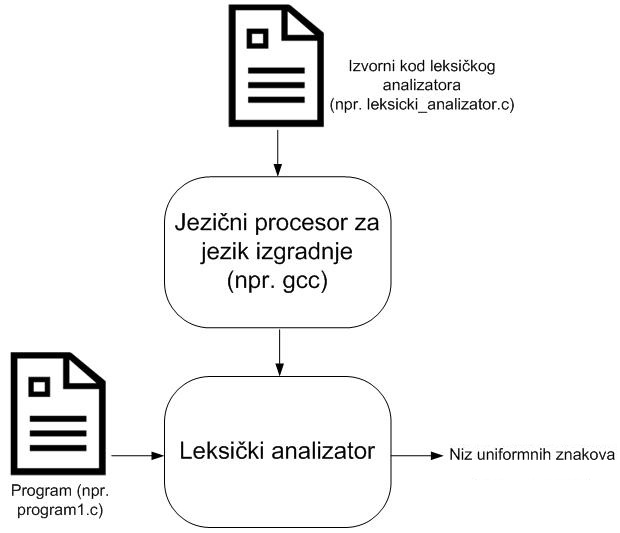
\includegraphics[width=0.7\textwidth]{slike/leksicki-analizator.jpg}
\caption{Način rada leksičkog analizatora.}
\label{fig:leksicki-analizator}
\end{figure}

Slika \ref{fig:leksicki-analizator} prikazuje dinamiku rada leksičkog analizatora.
Izvorni kod leksičkog analizatora dobiven primjenom izgrađenog generatora leksičkog analizatora treba prevesti u izvodivi oblik primjenom odgovarajućeg jezičnog procesora (ako je jezik izgradnje interpretirani jezik onda se ovaj korak preskače).
Izvodivi leksički analizator čita izvorni kod nekog programa pisanog u zadanom izvornom jeziku (na primjer jeziku \emph{C}) \emph{sa standardnog ulaza}.
Rezultat izvođenja leksičkog analizatora u jezičnom procesoru su \emph{niz uniformnih znakova} i \emph{tablica znakova}.

\subsection{Ispis leksičkog analizatora}
Za potrebe prve laboratorijske vježbe, leksički analizator \emph{na standardni izlaz} treba za svaki element niza uniformnih znakova ispisati redak sljedećeg oblika:\\
\\
\emph{uniformniZnak}\textvisiblespace\emph{redakPrograma}\textvisiblespace\emph{leksičkaJedinka}\\
\\
Pritom je \emph{uniformniZnak} odgovarajući uniformni znak iz Ulazne datoteke, \emph{redakPrograma} broj retka u ulaznom programu u kojem se leksička jedinka nalazi ako se \textbf{retci broje od 1} i \emph{leksičkaJedinka} je niz znakova ulaznog programa koji su grupirani u leksičku jedinku.
Ta tri dijela retka međusobno su odvojeni sa po jednim razmakom.
Primjer izlaza prikazan je u odjeljku \ref{sec:leksicki_analizator_primjer}.

\subsection{Strukture podataka leksičkog analizatora}
Leksički analizator na ulazu prima programski kod u jeziku opisanom Ulaznom Datotekom.
Kao rezultat, leksički analizator treba stvoriti niz uniformnih znakova i tablicu znakova (engl. \emph{symbol table}).
Zbog jednostavnosti Ulazne Datoteke, tablica znakova može biti jedino homogena, odnosno jedna tablica (kako god bila implementirana) sadržavat će na kraju rada leksičkog analizatora sve leksičke jedinke koje se nalaze u ulaznom programu.
Drugim rječima, Ulazna Datoteka ne omogućuje razvrstavanje simbola u tablicu ključnih riječi, tablicu konstanti i tablicu identifikatora.

Niz uniformnih znakova mora za svaku prepoznatu leksičku jedinku sadržavati ime leksičke jedinke, redak u kojem se ta jedinka nalazi u ulaznom programu i neku informaciju kako doći do odgovarajućeg zapisa u tablici znakova; to može biti pokazivač, indeks ili nešto treće.

Nakon završetka rada leksičkog analizatora, tablica znakova treba sadržavati točno jedan zapis za svaku leksičku jedinku u ulaznom programu.

\subsection{Algoritam leksičkog analizatora}
U udžbeniku su opisana dva algoritma leksičkog analizatora.
U poglavlju 2.9.6, opisan je algoritam zasnovan na DKA, a u poglavlju 2.9.7 algoritam zasnovan na \(\varepsilon\)-NKA.
Implementacijom algoritma zasnovanog na \(\varepsilon\)-NKA neće biti potrebno ostvarivati pretvorbu \(\varepsilon\)-NKA u DKA (koja je obrađena na predmetu “Uvod u teoriju računarstva”) te je stoga taj algoritam predložen za prvu laboratorijsku vježbu (vidi savjete za implementaciju).

\subsection{Razrješavanje nejednoznačnosti}
Generirani leksički analizator nejednoznačnost treba rješavati koristeći pravila P2 i P3 iz poglavlja 2.9.3 i 2.9.4 udžbenika (prioritet po duljini prepoznatog niza i prioritet po poretku pravila).

\subsection{Postupak oporavka od pogreške}
Za postupak oporavka od pogreše treba koristiti jednostavan postupak odbacivanja prvog znaka iz ulaznog programa kao što je opisano u poglavlju 2.9.5 udžbenika.
Prijavu pogrešaka obavljati isključivo na izlaz za greške (\emph{stderr}).
Dodatno, iako se u ispisu leksičkog analizatora eksplicitno ne navode greške niti nije vidljivo kako se analizator oporavlja od pogreške, ispravnost implementacije ovog postupka utjecat će na ispis za sve ulazne programe koji sadrže barem jednu leksičku pogrešku.

\subsection{Primjer}\label{sec:leksicki_analizator_primjer}
Kao nastavak prije obrađenog primjera, prikazat ćemo rezultat rada leksičkog analizatora generiranog za primjer u odjeljku \ref{sec:generator_primjer} ovih uputa, nad ulaznim programom koji je zbog preglednosti ponovljen u ispisu \ref{lst:minusLang_primjer_ponovljen}.

\begin{lstlisting}[caption={Primjer programa pisanog u jeziku \emph{minusLang}.},label=lst:minusLang_primjer_ponovljen]
#| ovo je primjer |#
3 -  -0x12 - ( #| ovdje ce doci grupirane
		operacije |#
3- -
--076) #| 3 - ---076 = 3 - -076 = 3 + 076 |#

\end{lstlisting}

Datoteka s ovim primjerom za potrebe testiranja može se pronaći \href{https://github.com/fer-ppj/ppj-labosi/raw/master/res/lab1/primjer.minus}{ovdje}.
Leksički analizator u skladu s ranije opisanom Ulaznom Datotekom generira sljedeći niz uniformnih znakova i tablicu znakova:

\begin{table}[ht]
\begin{minipage}[b]{0.5\linewidth}
\centering
\begin{tabular}{|l|c|c|}
\hline
uniformni znak&redak&indeks\\
\hline
OPERAND&2&0\\
\hline
OP\_MINUS&2&1\\
\hline
UMINUS&2&2\\
\hline
OPERAND&2&3\\
\hline
OP\_MINUS&2&1\\
\hline
LIJEVA\_ZAGRADA&2&4\\
\hline
OPERAND&4&0\\
\hline
OP\_MINUS&4&1\\
\hline
UMINUS&4&2\\
\hline
UMINUS&5&2\\
\hline
UMINUS&5&2\\
\hline
OPERAND&5&5\\
\hline
DESNA\_ZAGRADA&5&6\\
\hline
\end{tabular}
\end{minipage}
\hspace{0.5cm}
\begin{minipage}[b]{0.5\linewidth}
\centering
\begin{tabular}{|l|l|l|}
\hline
0&OPERAND&3\\
\hline
1&OP\_MINUS&-\\
\hline
2&UMINUS&-\\
\hline
3&OPERAND&0x12\\
\hline
4&LIJEVA\_ZAGRADA&(\\
\hline
5&OPERAND&076\\
\hline
6&DESNA\_ZAGRADA&)\\
\hline
\end{tabular}
\end{minipage}
\end{table}

U drugom stupcu niza uniformnih znakova naveden je redak u kojem se uniformni znak nalazi u ulaznoj datoteci.
U trećem stupcu naveden je indeks u tablicu znakova.

U ovom primjeru važno je uočiti dvije stvari.
Prvo, iako se operand \verb|3| u tekstu programa pojavljuje na dva mjesta, u tablici postoji samo jedan (zajednički) zapis jer se radi o dva pojavljivanja iste leksičke jedinke.
Drugo, iako se zapisi za binarni i unarni minus u tekstu programa ne razlikuju, u tablici znakova postoje zasebni zapisi za binarni i unarni minus zato jer se radi o različitim leksičkim jedinkama.

Očekivani ispis na standardni izlaz prikazan je \href{https://github.com/fer-ppj/ppj-labosi/raw/master/res/lab1/minus_primjer_izlaz.txt}{ovdje}.
Treba uočiti da ispis završava praznim retkom tj.~da svi retci (osim tog praznog) završavaju znakom kraja retka.

\section{Način računalnog ocjenjivanja rješenja}
Za potrebe računalnog ocjenjivanja rješenje prve laboratorijske vježbe treba predati u jednoj \emph{zip} datoteci.
U korijenskom direktoriju trebaju se nalaziti \textbf{sve} datoteke s izvornim kodom \textbf{generatora} leksičkog analizatora.
Korijenski direktorij \emph{zip} datoteke mora sadržavati poddirektorij \texttt{analizator}.
Poddirektorij \texttt{analizator} može inicijalno sadržavati dijelove implementacije leksičkog analizatora koji ne ovise o Ulaznoj datoteci, ali i ne mora sadržavati ništa.
Na primjer, za rješenje u jeziku \emph{C}, sadržaj \emph{zip} datoteke mogao bi izgledati kao u ispisu \ref{lst:gla_zip_struktura}.

\begin{lstlisting}[caption={Primjer sadržaja \emph{zip} datoteke. Imena datoteka \emph{nisu važna}.},label=lst:gla_zip_struktura]
analizator/bar.c
analizator/bar.h
analizator/lekser.h
analizator/predlozak.txt
foo.c
foo.h
generator.c
\end{lstlisting}

Za prevođene jezike izgradnje, sustav za računalno ocjenjivanje će prevesti predane datoteke u izvodivi oblik generatora leksičkog analizatora u korijenskom direktoriju.
Za prethodni primjer, rezultat bi mogao izgledati kao u ispisu \ref{lst:gla_preveden}.

\begin{lstlisting}[caption={Primjer sadržaja korijenskog direktorija nakon prevođenja generatora.},label=lst:gla_preveden]
analizator/bar.c
analizator/bar.h
analizator/lekser.h
analizator/predlozak.txt
foo.c
foo.h
generator.c
generator.exe
\end{lstlisting}

Generatoru leksičkog analizatora na standardni ulaz se predaje opis procesa leksičkog analizatora, a generator priprema izvorni kod leksičkog analizatora u poddirektoriju \texttt{analizator}, kao u ispisu \ref{lst:la_pripremljen}.
Važno je uočiti da se \emph{izlaz generatora} ne provjerava izravno --- generator ne mora ispisati ništa, ali mora pripremiti tj.~generirati analizator.

\begin{lstlisting}[caption={Primjer sadržaja korijenskog direktorija nakon izvođenja generatora.},label=lst:la_pripremljen]
analizator/bar.c
analizator/bar.h
analizator/lekser.h
analizator/lekser.c
analizator/predlozak.txt
analizator/tablica.txt
foo.c
foo.h
generator.c
generator.exe
\end{lstlisting}

Nakon izvođenja generatora leksičkog analizatora, u poddirektoriju \texttt{analizator} mora se nalaziti sav potrebni izvorni kod za prevođenje leksičkog \textbf{analizatora}.
Sustav će prevesti datoteke u poddirektoriju u izvodivi oblik leksičkog analizatora u istom poddirektoriju, kao što je prikazano u ispisu \ref{lst:la_preveden}.

\begin{lstlisting}[caption={Primjer sadržaja korijenskog direktorija nakon izvođenja generatora.},label=lst:la_preveden]
analizator/analizator.exe
analizator/bar.c
analizator/bar.h
analizator/lekser.h
analizator/lekser.c
analizator/predlozak.txt
analizator/tablica.txt
foo.c
foo.h
generator.c
generator.exe
\end{lstlisting}

Konačno, izvodivi leksički analizator na standardni ulaz dobiva izvorni kod programa i treba ispisati rezultat izvođenja kao što je ranije opisano.

Uočite da su \textbf{generator} i \textbf{analizator} dva \emph{odvojena programa}.
Nije dozvoljeno kopirati Ulaznu datoteku u "generatoru" i onda ju ponovno parsirati u "analizatoru", stvarati automate i tek onda analizirati ulazni program.
Generator je taj program koji mora završiti definiciju analizatora.
To se, na primjer, može ostvariti tako da generator generira programski kod koji u analizatoru inicijalizira tablice automata ili da generira datoteku s tablicama automata koju onda analizator čita.

Za rješenja u \emph{Javi} i \emph{C\#}-u, ulazna točka u generator \textbf{mora biti} u razredu \texttt{GLA}, a ulazna točka u analizator u razredu \texttt{LA}.
Za rješenja u \emph{Pythonu}, za izvođenje generatora će se pozvati datoteka \texttt{GLA.py}, a za izvođenje analizatora datoteka \texttt{LA.py}.

Detalji oko predaje, kao što su inačice alata koji će se koristiti za prevođenje i izvođenje rješenja, bit će objavljeni naknadno na FERWebu.

\section{Savjeti za implementaciju}
Savjeti za implementaciju navedeni u ovom poglavlju zamišljeni su kao pomoć u izradi generatora leksičkog analizatora.
Kao takvi, nisu obvezujući i grupe po vlastitom nahođenju mogu dio ili sve savjete u ovom poglavlju zanemariti.

\subsection{Generiranje koda leksičkog analizatora}
Veliki dio izvornog koda generiranog leksičkog analizatora neovisan je od Ulazne Datoteke i treba biti napisan unaprijed.
Preporuča se da se taj dio koda zasebno razvije i testira, na primjer koristeći izmišljenu tablicu konačnog automata.
Na taj način, generator leksičkog analizatora može razvijeni kod iskopirati u datoteku s izvornim kodom leksičkog analizatora i dopuniti datoteku definicijom tablice konačnog automata i slično.

\subsection{Priprema regularnih izraza za generiranje konačnog automata}
Prije generiranja \(\varepsilon\)-NKA iz regularnog izraza, potrebno je sve regularne definicije koji se pojavljuju u regularnom izrazu zamijeniti odgovarajućim regularnim izrazima.
S obzirom na ograničenja regularnih definicija, svaka regularna definicija će prije njenog referenciranja biti definirana.
Prema tome, zamjena regularnih definicija se tijekom rada generatora leksičkog analizatora može obaviti algoritmom prikazanim u pseudokodu u ispisu \ref{lst:priprema_regexa}.

\begin{lstlisting}[caption={Pseudokod za pripremu regularnih izraza za generiranje konačnog automata.},label=lst:priprema_regexa]
za svaku regularnu definiciju {regDef} u Ulaznoj Datoteci
	neka je regEx regularni izraz koji opisuje definicjiu {regDef}
	za svaku referencu {refRegDef} u regularnom izrazu regEx
		zamijeni {refRegDef} u izrazu regEx s
           "(" + regularniIzraz[{refRegDef}] + ")"
	regularniIzraz[{regDef}] = regEx
\end{lstlisting}

Ključno je primijetiti da se koristeći ovaj algoritam svakoj regularnoj definiciji neposredno nakon što je pročitana iz Ulazne Datoteke pridruži "čisti" regularni izraz koji ne referencira niti jednu regularnu definiciju.
Također, kako bi se očuvala očekivana prednost operatora, nužno je prije zamjene regularni izraz koji opisuje neku regularnu definiciju okružiti zagradama.
Koristeći vrlo sličan algoritam i "čiste" regularne izraze za regularne definicije, moguće je pripremiti sve regularne izraze iz Ulazne Datoteke za generiranje konačnog automata, tj.~zamijeniti sve reference na regularne definicije odgovarajućim regularnim izrazom.

Na primjer, neka su zadane sljedeće regularne definicije:\\
\verb={znamenka} 0|1|2|3|4|5|6|7|8|9=\\
\verb={hexZnamenka} {znamenka}|a|b|c|d|e|f|A|B|C|D|E|F=

Regularni izraz za regularnu definiciju \verb|{znamenka}| ne sadrži reference na niti jednu regularnu definiciju.
Regularni izraz za definiciju \verb|{hexZnamenka}| sadrži referencu na definiciju \verb|{znamenka}| tako da će primjenom opisanog algoritma regularni izraz za definiciju \verb|{hexZnamenka}| biti preveden u \verb=(0|1|2|3|4|5|6|7|8|9)|a|b|c|d|e|f|A|B|C|D|E|F=

Kada bi u dijelu pravila bilo definirano pravilo:\\
\verb=<S_nekoStanje>0x{hexZnamenka}{hexZnamenka}*=\\
\verb={=\\
\verb=HEX_KONSTANTA=\\
\verb=}=\\
uvrštavanjem takvog regularnog izraza za definiciju \verb|{hexZnamenka}| dobili bi jednostavan regularan izraz za prikazano pravilo (oba retka dio su istog izraza):\\
\verb=0x((0|1|2|3|4|5|6|7|8|9)|a|b|c|d|e|f|A|B|C|D|E|F)=\\
\verb=((0|1|2|3|4|5|6|7|8|9)|a|b|c|d|e|f|A|B|C|D|E|F)*=

Ovakav regularni izraz može se prevesti u \(\varepsilon\)-NKA koristeći ranije spomenuti algoritam opisan u udžbeniku "Uvod u teoriju računarstva" \cite[poglavlje 2.2.2]{utr}.

\subsection{Izgradnja $\varepsilon$-NKA iz regularnih izraza za potrebe leksičkog analizatora}
Ako se u obradi referenci na regularne definicije koristi algoritam koji je opisan u prethodnom poglavlju, za regularne izraze definicija nije potrebno graditi konačne automate jer se ti regularni izrazi na tekstualnoj razini umeću u regularne izraze pravila.

Kao što je navedeno u opisu pravila, svako pravilo bit će pridruženo točno jednom stanju leksičkog analizatora.
Implementacija generatora mora osigurati da generirani leksički analizator koristi isključivo ona pravila koja su aktivna u trenutnom stanju leksičkog analizatora.
To ograničenje moguće je ostvariti tako da se za svako stanje leksičkog analizatora generira zaseban \(\varepsilon\)-NKA te se ulazni znakovi predaju samo automatu koji je zadužen za obradu trenutno aktivnog stanja leksičkog analizatora.

Postupak izgradnje \(\varepsilon\)-NKA za potrebe leksičkog analizatora opisan je u udžbeniku \cite[poglavlje 2.9.2]{udzbenik}.
Bitno je primijetiti da je prilikom dodavanja početnog stanja \(p_0\) (vidi udžbenik) i spajanja svih automata \(M_i\) u jedinstveni automat nužno osigurati da sva stanja u automatima \(M_i\) imaju jedinstvene oznake.
U suprotnom automat vrlo vjerojatno neće raditi ispravno!
Kako bi se izbjegla potreba za preimenovanjem stanja, moguće je umjesto spajanja automata \(M_i\) u jedinstveni automat za neko stanje leksičkog analizatora automate \(M_i\) pohraniti odvojeno.
Na taj način će svako pravilo pridruženo nekom stanju leksičkog analizatora imati svoj \(\varepsilon\)-NKA.
Ova promjena utječe na sam algoritam rada leksičkog analizatora opisan u \cite[poglavlje 2.9.7]{udzbenik} jer će leksički analizator umjesto jednog koristiti nekoliko \(\varepsilon\)-NKA.

Izgradnja \(\varepsilon\)-NKA za regularni izraz svakog pravila načelno je opisana u udžbeniku predmeta "Uvod u teoriju računarstva".
S obzirom na to da je postupak relativno složen, a nije središnja tema ove laboratorijske vježbe, u nastavku je dan pseudokod koji opisuje jedan način na koji se pretvorba može ostvariti.

Funkciji u pseudokodu predaje se regularni izraz i automat koji treba izgraditi.
Vizualno, automat se gradi s lijeva na desno pa se imena varijabli naslanjaju na tu predodžbu.
Funkcija kao rezultat vraća "lijevo" i "desno" stanje automata.
Lijevo stanje za cijeli izraz odgovara početnom stanju automata, a desno stanje za cijeli izraz odgovara prihvatljivom stanju automata.
Algoritam izgradnje \(\varepsilon\)-NKA iz regularnog izraza jamči da će automat imati točno jedno prihvatljivo stanje.
Poziv algoritma prikazan je u ispisu \ref{lst:regex_pseudo_poziv}.

\begin{lstlisting}[caption={Poziv funkcije \texttt{pretvori}.},label=lst:regex_pseudo_poziv]
ParStanja rezultat = pretvori(regularni_izraz, automat)
automat.pocetno_stanje = rezultat.lijevo_stanje
automat.prihvatljivo_stanje = rezultat.desno_stanje
\end{lstlisting}

Stanja automata označavat će se cijelim brojevima od nula na više.
Za dodavanje stanja automatu koristit će se funkcija \verb|novo_stanje|.
Funkcija \verb|novo_stanje| vraća oznaku dodanog stanja.
Pretpostavlja se da će početni broj stanja automata biti nula.
Pseudokod funkcije \verb|novo_stanje| prikazan je u ispisu \ref{lst:regex_pseudo_novo_stanje}.

\begin{lstlisting}[caption={Pseudokod funkcije za dodavanje stanja automatu.},label=lst:regex_pseudo_novo_stanje]
int novo_stanje(automat)
	automat.br_stanja = automat.br_stanja + 1
	vrati automat.br_stanja - 1
\end{lstlisting}

Prvi korak algoritma je potraga za operatorima izbora koji se nalaze izvan svih zagrada.
Operator izbora ima najnižu pretpostavljenu prednost od svih operatora koje koristimo u regularnim izrazima pa je zbog toga nužno kao prvi korak niz podijeliti na podnizove između kojih se može birati.
Na primjer, u regularnom izrazu\\
\verb=(\)a|b)\|\(|x*|y*=\\
postoje dva operatora izbora izvan svih zagrada (neposredno ispred \verb|x| i neposredno ispred \verb|y|).
Rezultat prvog koraka algoritma bila bi tri nova regularna izraza\\
\verb=(\)a|b)\|\(=\\
\verb|x*|\\
\verb|y*|

Traženje operatora izbora izvan svih zagrada zahtijeva brojanje zagrada s lijeva na desno.
Brojač zagrada kreće od \verb|0|, povećava se za jedan za svaku otvorenu zagradu, a smanjuje za jedan za svaku zatvorenu zagradu.
Ako algoritam naiđe na operator izbora kada je brojač zagrada jednak nuli, preostali dio izraza podijeli oko operatora izbora i nastavi dalje prema desno.
Iz primjera je očito da pritom posebnu pažnju treba posvetiti zagradama i operatorima izbora koji su prefiksirani znakom \verb|\| i nemaju svoje originalno značenje.
Općenito, nužno je provjeriti nalazi li se ispred određenog operatora paran ili neparan broj znakova \verb|\|.
U algoritmu pretvorbe koristit će se pomoćna funkcija \verb|je_operator| koja za dani regularni izraz i indeks operatora provjerava ima li operator svoje značenje ili je prefiksiran neparnim brojem znakova \verb|\|.
Pseudokod funkcije \verb|je_operator| prikazan je u ispisu \ref{lst:regex_pseudo_je_operator}.

\begin{lstlisting}[caption={Pseudokod funkcije \texttt{je\_operator}.},label=lst:regex_pseudo_je_operator]
bool je_operator(izraz, i)
	int br = 0
	dok je i-1>=0 && izraz[i-1]=='\\' // jedan \, kao u C-u
	    br = br + 1
	    i = i - 1
	kraj dok
	vrati br%2 == 0
\end{lstlisting}

Dio funkcije \verb|pretvori| koji broji zagrade i dijeli izraz na podizraze odvojene operatorom izbora prikazan je u ispisu \ref{lst:regex_pseudo_pretvori_1}.

\begin{lstlisting}[caption={Početak funkcije \texttt{pretvori}.},label=lst:regex_pseudo_pretvori_1]
ParStanja pretvori(izraz, automat)
	niz izbori
	int br_zagrada = 0
	za (i=0; i<duljina(izraz); i=i+1)
	  ako je izraz[i]=='(' && je_operator(izraz, i)
	    br_zagrada = br_zagrada + 1
	  inace ako je izraz[i]==')' && je_operator(izraz, i)
	    br_zagrada = br_zagrada - 1
	  inace ako je br_zagrada==0 && izraz[i]=='|' && je_operator(izraz, i)
	    grupiraj lijevi negrupirani dio niza znakova izraz u niz izbori
	  kraj ako
	kraj za
	ako je pronadjen barem jedan operator izbora
	  grupiraj preostali negrupirani dio niza znakova izraz u niz izbori
	...
\end{lstlisting}

Nakon ovog odsječka, moguće je da je u nizu pronađen neki broj operatora izbora ili da se izraz na najvišoj razini (dakle, izvan svih zagrada) sastoji samo od podizraza povezanih nadovezivanjem.
Nastavak algoritma koji započinje izgradnja automata prikazan je u ispisu \ref{lst:regex_pseudo_pretvori_2}.

\begin{lstlisting}[caption={Nastavak funkcije \texttt{pretvori}.},label=lst:regex_pseudo_pretvori_2]
    ...
    int lijevo_stanje = novo_stanje(automat)
    int desno_stanje = novo_stanje(automat)
    ako je pronadjen barem jedan operator izbora
        za (i=0; i<br_elemenata(izbori); i=i+1)
          ParStanja privremeno = pretvori(izbori[i], automat)
          dodaj_epsilon_prijelaz(automat,
             lijevo_stanje,         
             privremeno.lijevo_stanje)
          dodaj_epsilon_prijelaz(automat,
                              privremeno.desno_stanje,
                              desno_stanje)
        kraj za
    inace
      ...
\end{lstlisting}

Kao što je prikazano odsječkom u ispisu \ref{lst:regex_pseudo_pretvori_2}, ako su u izrazu pronađeni podizrazi odvojeni operatorom izbora, svaki podizraz se rekurzivno obradi pozivom funkcije \verb|pretvori| i lijeva i desna stanja dobivena od rekurzivnog poziva povežu se epsilon prijelazima s lijevim i desnim stanjem za cijeli izraz.
Ovaj postupak je poopćenje točke \emph{p4} u \cite[poglavlje 2.2.2]{utr}.
U ispisu \ref{lst:regex_pseudo_pretvori_3} je opisana obrada drugog slučaja u kojem nisu pronađeni operatori izbora.

\begin{lstlisting}[caption={Obrada nadovezivanja u funkciji \texttt{pretvori}.},label=lst:regex_pseudo_pretvori_3]
      ... // nastavlja se inace iz proslog odsjecka
      bool prefiksirano = laz
      int trenutno_stanje = lijevo_stanje
      za (i=0; i<duljina(izraz); i=i+1)
        ako je prefiksirano istina
          *slucaj 1*
        inace
          *slucaj 2*
        kraj ako
      kraj za
      dodaj_epsilon_prijelaz(automat, trenutno_stanje, desno_stanje)
\end{lstlisting}

Varijabla \verb|prefiksirano| služi za prepoznavanje je li trenutni znak u izrazu prefiksiran znakom \verb|\|.
Varijabla \verb|trenutno_stanje| sadrži broj najdesnijeg stanja u postupku izgradnje automata.
Kao što je prije spomenuto, postupak kreće s lijeva na desno.
Na kraju obrade cijelog izraza (zadnja linija pseudokoda), najdesnije generirano stanje povezuje se epsilon prijelazom s desnim stanjem koje će se vratiti na kraju funkcije.
Pri obradi svakog znaka izraza postoje dva slučaja, ovisno o tome je li znak prefiksiran znakom \verb|\| ili nije.
Pseudokod za \emph{slučaj 1} prikazan je u ispisu \ref{lst:regex_pseudo_slucaj_1}.

\begin{lstlisting}[caption={Slučaj 1 u funkciji \texttt{pretvori}.},label=lst:regex_pseudo_slucaj_1]
// slucaj 1
prefiksirano = laz
char prijelazni_znak
ako je izraz[i] == 't'
  prijelazni_znak = '\t' // jedan znak, kao u C-u
inace ako je izraz[i] == 'n'
  prijelazni_znak = '\n' // jedan znak, kao u C-u
inace ako je izraz[i] == '_'
  prijelazni_znak = ' ' // obican razmak
inace
  prijelazni_znak = izraz[i]
kraj ako

int sljedece_stanje = novo_stanje(automat)
dodaj_prijelaz(automat, trenutno_stanje, sljedece_stanje, 
    prijelazni_znak)
*provjeri ponavljanje*
trenutno_stanje = sljedece_stanje
\end{lstlisting}

Odsječak za slučaj 1 prvo postavlja varijablu \verb|prefiksirano| u laž zato jer je prefiks iz prošlog znaka potrošen na znak koji se trenutno obrađuje.
Ograničenja na Ulaznu Datoteku osiguravaju da će u slučaju 1 \verb|izraz[i]| biti neki od specijalnih znakova opisanih u ovoj uputi u odjeljku \ref{sec:specijalni_znakovi}.
Posebnu pažnju treba posvetiti znakovima za tab, novi redak i prazninu.
Prijelazni znak u automatu treba biti onaj znak kojeg će leksički analizator pročitati u ulaznom programu.
Nakon što je određen prijelazni znak, automatu se dodaje novo stanje i odgovarajući prijelaz. 

Provjera za operator ponavljanja odvojena je jer će se ponoviti nekoliko puta u cijelom pseudokodu.
Ponavljanje se prevodi u automat slično kao u točki \emph{p6} u \cite[poglavlje 2.2.2]{utr}.
Pseudokod je prikazan u ispisu \ref{lst:regex_pseudo_ponavljanje}.

\begin{lstlisting}[caption={Obrada ponavljanja Kleenovim operatorom.},label=lst:regex_pseudo_ponavljanje]
// provjeri ponavljanje
ako je i+1<duljina(izraz) && izraz[i+1]=='*'
  dodaj_epsilon_prijelaz(automat, trenutno_stanje, sljedece_stanje)
  dodaj_epsilon_prijelaz(automat, sljedece_stanje, trenutno_stanje)
  i = i+1
kraj ako
\end{lstlisting}

Nakon dodavanja epsilon prijelaza koji obrađuju ponavljanje, znak ponavljanja se preskače pomicanjem indeksa za jedan unaprijed.

Obrada slučaja 2 u kojem znak nije prefiksiran znakom \verb|\| prikazana je u ispisu \ref{lst:regex_pseudo_slucaj_2}.

\begin{lstlisting}[caption={Slučaj 2 u funkciji \texttt{pretvori}.},label=lst:regex_pseudo_slucaj_2]
// slucaj 2
ako je izraz[i] == '\\' // jedan znak \, kao u C-u
  prefiksirano = istina
  nastavi za petlju // continue u C-u
kraj ako
ako je izraz[i] != '('
  *slucaj 2a*
inace
  *slucaj 2b*
kraj ako
\end{lstlisting}

U slučaju 2, prvo se provjerava je li trenutni znak baš znak \verb|\|.
Ako je, postavlja se varijabla prefiksirano i prelazi se na sljedeći znak.
U suprotnom, provjerava se je li trenutni znak otvorena zagrada koja započinje neki podizraz.
Time se slučaj dijeli na dva podslučaja.
Ako trenutni znak nije otvorena zagrada onda se sigurno radi o nekom znaku kojeg treba nadovezati na dosad izgrađeni automat.
Pseudokod za ovaj slučaj prikazan je u ispisu \ref{lst:regex_pseudo_slucaj_2a}.

\begin{lstlisting}[caption={Slučaj 2a u funkciji \texttt{pretvori}.},label=lst:regex_pseudo_slucaj_2a]
// slucaj 2a
int sljedece_stanje = novo_stanje(automat)
ako je izraz[i] == '$'
  dodaj_epsilon_prijelaz(automat, trenutno_stanje, sljedece_stanje)
inace
  dodaj_prijelaz(automat, trenutno_stanje, sljedece_stanje, izraz[i])
kraj ako
*provjeri ponavljanje*
trenutno_stanje = sljedece_stanje
\end{lstlisting}

Posebna pažnja pridaje se znaku \verb|$| koji označava prazan niz.
Dodatno, nakon obrade znaka provjerava se postoji li nakon znaka operator ponavljanja.

Konačno, slučaj 2b pokriva mogućnost podizraza ograđenog zagradama.
Pseudokod za ovaj slučaj prikazan je u ispisu \ref{lst:regex_pseudo_slucaj_2b}.

\begin{lstlisting}[caption={Slučaj 2b u funkciji \texttt{pretvori}.},label=lst:regex_pseudo_slucaj_2b]
// slucaj 2b
int j = *pronadji odgovarajucu zatvorenu zagradu*
ParStanja privremeno = pretvori(izraz[i+1..j-1], automat)
dodaj_epsilon_prijelaz(automat, trenutno_stanje,
    privremeno.lijevo_stanje)
i = j
trenutno_stanje = privremeno.desno_stanje
ako je i+1<duljina(izraz) && izraz[i+1]=='*'
  dodaj_epsilon_prijelaz(automat, privremeno.lijevo_stanje, privremeno.desno_stanje)
  dodaj_epsilon_prijelaz(automat, privremeno.desno_stanje, privremeno.lijevo_stanje)
  i = i+1
kraj ako
\end{lstlisting}

Traženje odgovarajuće zatvorene zagrade može se obaviti brojeći zagrade na vrlo sličan način kao na početku funkcije pretvori pa ovdje neće biti opisano.
Kada je pronađena zatvarajuća zagrada, izraz u zagradi rekurzivno se obradi i poveže s trenutno najdesnijim stanjem epsilon prijelazom.
Konačno, provjeri se postoji li operator ponavljanja.
Ostvarenje ponavljanja koristi različite varijable u odnosu na prethodna dva slučaja pa je ovdje posebno navedeno da se izbjegne zabuna.

Funkcija \verb|pretvori| na kraju vraća vrijednosti varijabli \verb|lijevo_stanje| i \verb|desno_stanje| u strukturi \verb|ParStanja|.
Cijeli pseudokod u jednoj datoteci može se naći \href{https://github.com/fer-ppj/ppj-labosi/raw/master/res/lab1/regex_pseudokod.txt}{ovdje}.

\subsection{Ostvarenje tablice znakova}
Kroz treću laboratorijsku vježbu, zapisi u tablici znakova morat će se proširivati dodatnim podacima.
Za prvu laboratorijsku vježbu to znači da je poželjno sve pristupe tablici znakova ostvariti kroz pomoćne funkcije ili metode tako da kasnije bude moguće potrebne promjene obaviti na što manjem broju mjesta.
Dodatno, tablica znakova tijekom kasnijih faza rada jezičnog procesora može i rasti.
Na primjer, leksička analiza stvara jedan zapis u tablici znakova za svaku pojavu nekog identifikatora "x" u izvornom programu.
Međutim, ako se spomenuti identifikator pojavljuje u različitim kontekstima (na primjer, negdje se radi o \verb|int|, a negdje o \verb|char| varijabli), bit će nužno u tablicu znakova dodati zapise koji opisuju te različite instance identifikatora jednakog imena.

Alternativno, moguće je u kasnijim fazama rada koristiti više tablica znakova, ali o tome će više riječi biti u trećoj laboratorijskoj vježbi.

\section{Leksička analiza podskupa jezika \emph{C}}
Koristeći generator leksičkog analizatora potrebno je generirati leksički analizator za zadani podskup jezika \emph{C}.
Ulazna Datoteka koja definira taj leksički analizator može se naći \href{https://github.com/fer-ppj/ppj-labosi/raw/master/res/lab1/simplePpjLang.lan}{ovdje}.
Generirani leksički analizator će prepoznati ključne riječi jezika \emph{C} navedene u tablici \ref{tab:kljucne_rijeci}.

\begin{table}[ht]
\centering
\begin{tabular}{l l l}
\verb|break|&\verb|else|&\verb|return|\\
\verb|char|&\verb|for|&\verb|void|\\
\verb|const|&\verb|if|&\verb|while|\\
\verb|continue|&\verb|int|&
\end{tabular}
\caption{Podržane ključne riječi.}
\label{tab:kljucne_rijeci}
\end{table}

Podržani su cijeli brojevi u dekadskom, oktalnom i heksadekadskom zapisu.
Znakovne konstante i nizovi znakova zapisuju se jednako kao u jeziku \emph{C}.
Dozvoljeni su komentari koji započinju znakovima \verb|//| i traju do kraja retka i komentari koji su omeđeni nizovima \verb|/*| i \verb|*/|.

Generirani analizator će prepoznati specijalne znakove iz jezika \emph{C} navedene u tablici \ref{tab:specijalni_znakovi}.
\begin{table}[ht]
\centering
\begin{tabular}{l l l l l l l l l l l}
\verb|[|&\verb|]|&\verb|(|&\verb|)|&\verb|{|&\verb|}|&\verb|;|&\verb|,|&\verb|=|&&\\
\verb|++|&\verb|--|&\verb|&|&\verb=|=&\verb|*|&\verb|+|&\verb|-|&\verb|~|&\verb|!|&&\\
\verb|/|&\verb|%|&\verb|<|&\verb|>|&\verb|<=|&\verb|>=|&\verb|==|&\verb|!=|&\verb|^|&\verb|&&|&\verb=||=
\end{tabular}
\caption{Podržani specijalni znakovi.}
\label{tab:specijalni_znakovi}
\end{table}

Točno značenje pojedinog specijalnog znaka (npr.~radi li se o binarnom ili unarnom minusu) odredit će se tijekom kasnijih faza rada jezičnog procesora.
Primjer programa koji ispituje većinu leksičkih zahtjeva ovog podskupa jezika \emph{C} može se naći \href{https://github.com/fer-ppj/ppj-labosi/raw/master/res/lab1/primjer.simple}{ovdje}.
Leksički analizator bi trebao javiti tri greške u retku 27 i odbaciti sva tri apostrofa (jednog po jednog) u postupku oporavka od pogreške\footnote{Kao što je prije spomenuto, pripazite da leksički analizator ne ispisuje \textbf{ništa} na standardni izlaz osim traženog ispisa - greške ispisujte npr.~na \texttt{stderr}.}.
Očekivani izlaz za dani primjer prikazan je \href{https://github.com/fer-ppj/ppj-labosi/raw/master/res/lab1/simple_primjer_izlaz.txt}{ovdje}.

\newpage
\addcontentsline{toc}{chapter}{Literatura}
\begin{thebibliography}{10}
\bibitem{udzbenik}
Siniša Srbljić:
\emph{Prevođenje programskih jezika}, Element, 2007.
\bibitem{utr}
Siniša Srbljić:
\emph{Uvod u teoriju računarstva}, Element, 2007.
\end{thebibliography}

\end{document}
